% !TeX encoding = UTF-8
% !TeX spellcheck = en_US
% !TeX root = ../../Thesis.tex
\chapter{Electron beam setup}\label{ch:Electron beam setup}

chapter about electron beam setup

Charakterisierung der intakten CRT -> Frank 
Charakterisierung HVPS ->  Frank 

Skizze inkl. externe Power Supplies, wie wird die CRT betrieben?

Heater
Wie sieht der Innen aus? 
CRT Mount ??

\section{Charatarization of a working CRT}\label{sec:Charatarization of a working CRT}

HAMEG HM507 oscilloscopes were used for testing purposes. These contain a D14-363GY/123\autocite{tubedata} CRT hereinafter abbreviated as `D14', `tube', or `CRT'. Although the HM507 has only a bandwidth of \SIrange{0}{50}{\mega\hertz}, which is not sufficient for the hyperfine splitting frequency of \SI{461.7}{\mega\hertz}\todo{http://www.tobiastiecke.nl/archive/PotassiumProperties.pdf} of $^{39}\mathrm{K}$, it was used nevertheless because of its simple construction and availability. A schematic view of the device is shown in \cref{fig:electrode configuration} with the back pin arrangement in \cref{fig:pin arrangement}.

The voltages and currents of the necessary pins to drive the CRT were measured with a voltage probe \todo{model number} with an attenuation ratio of \todo{1:100 or 100:1} and are summarized in \cref{tab:D14-363GY/123 tube pin measurements}. It was not possible to measure pin g3 directly. Therefore a HVPS (\cref{sec:HVPS}) was used to set a voltage and the beam diameter was observed. The best focus was achieved with a voltage of \SI{-1.813e3}{\volt}.

\begin{figure}[H]
	\centering
	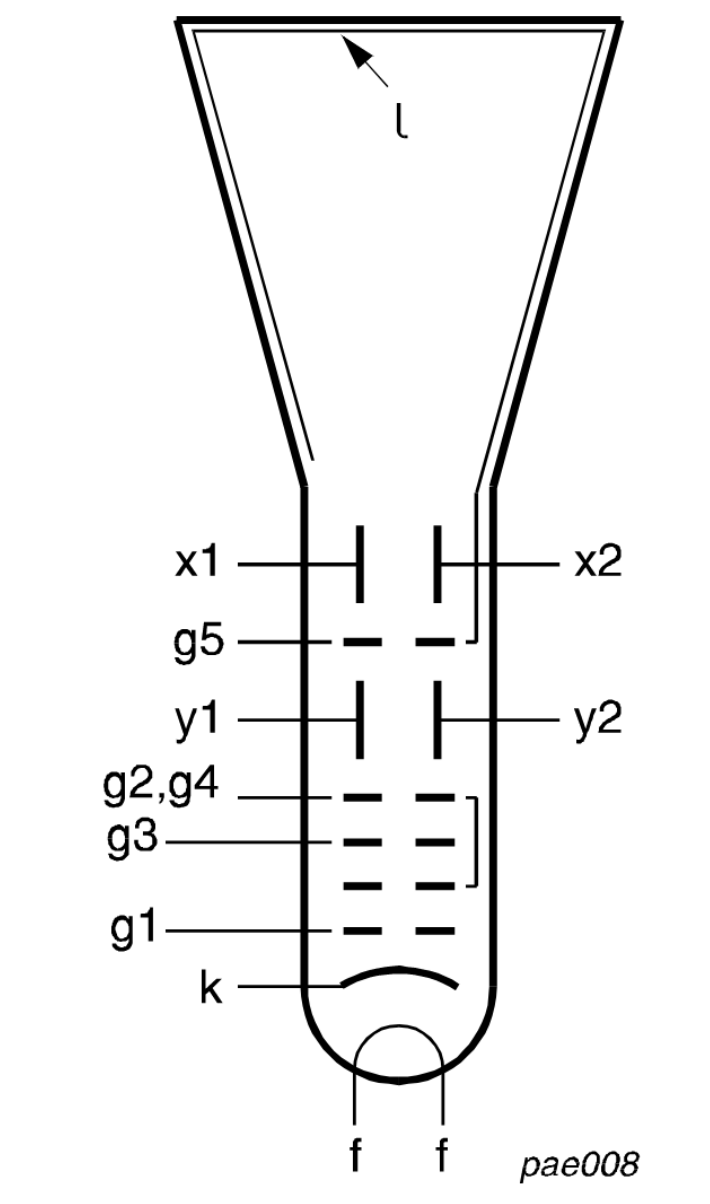
\includegraphics[width=5cm]{./Chapters/e-beam-setup/electrode configuration}
	\caption{Electrode configuration (from \autocite{tubedata})}
	\todo[inline]{how to cite figure}
	\label{fig:electrode configuration}
\end{figure}

\begin{figure}[H]
	\centering
	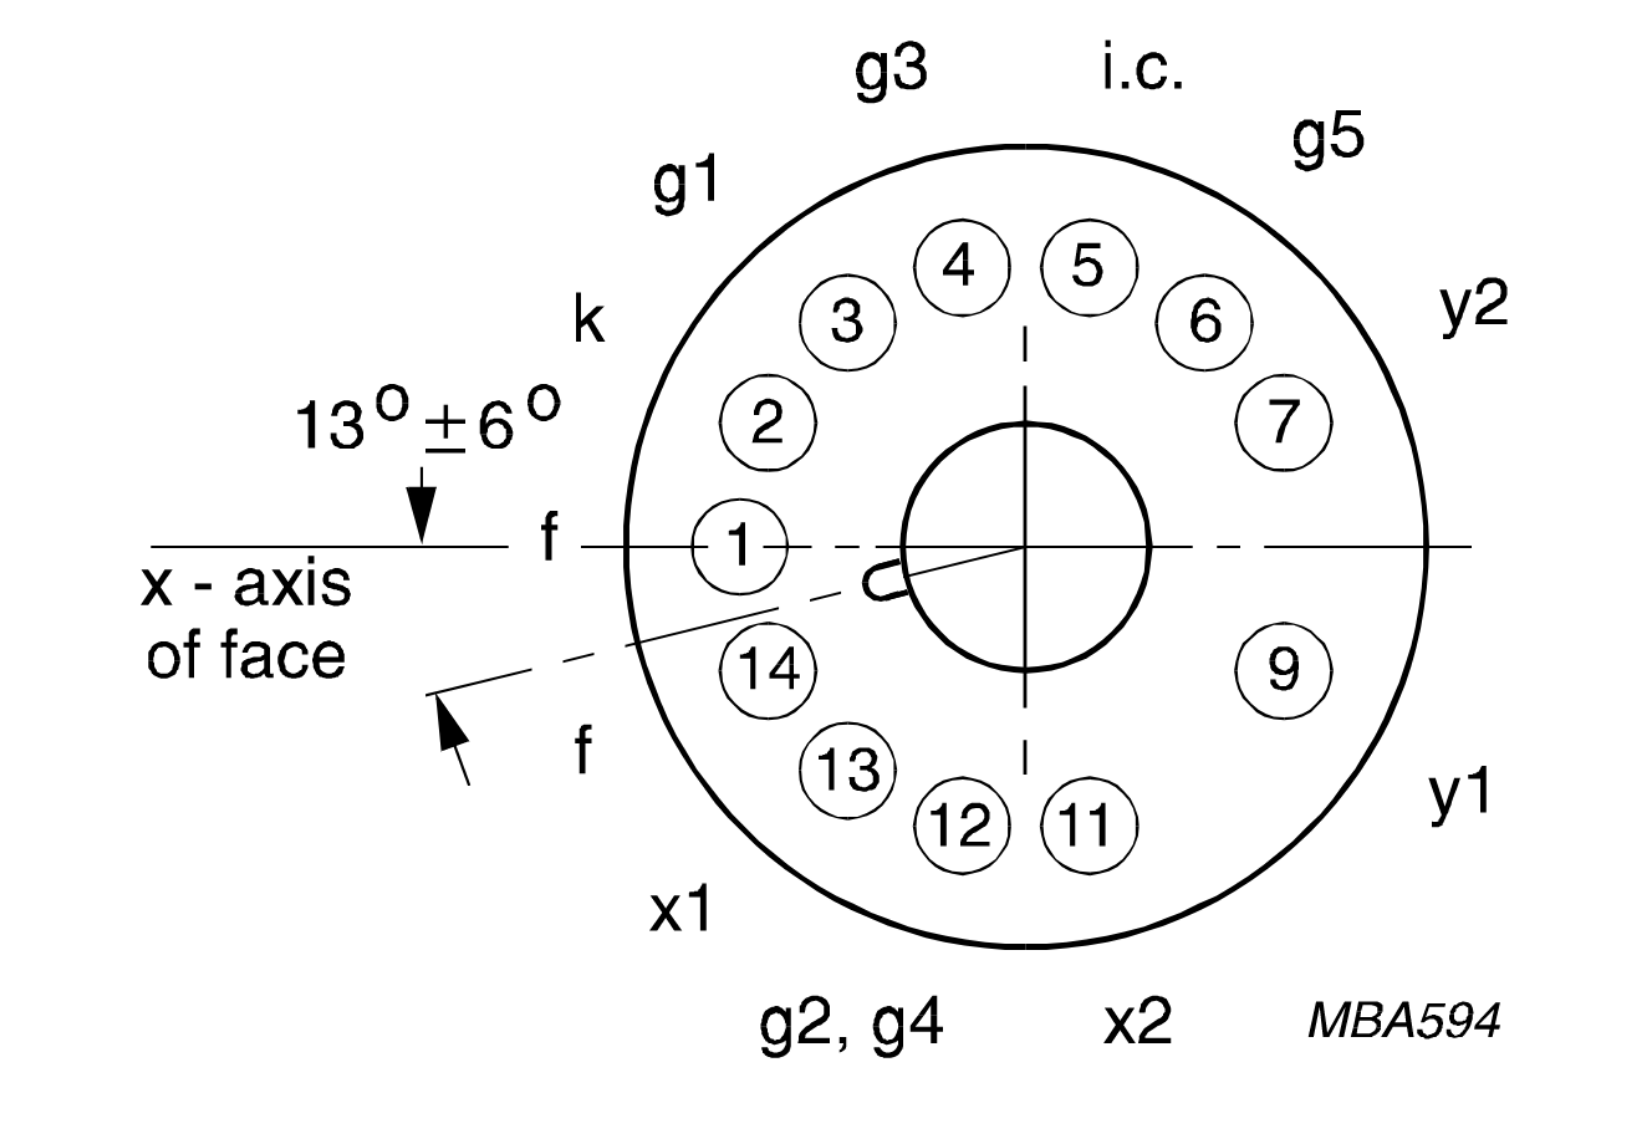
\includegraphics[width=5cm]{./Chapters/e-beam-setup/pin arrangement}
	\caption{Pin arrangement, bottom view (from \autocite{tubedata})}
	\todo[inline]{how to cite figure}
	\label{fig:pin arrangement}
\end{figure}


\begin{table}[H]
	\centering
	\caption{D14-363GY/123 CRT pin measurements}
	\label{tab:D14-363GY/123 tube pin measurements}
	\begin{tabular}{S c *{2}{S}}
		\toprule
		{number} & {pin}  & {voltage/\si{\volt}} & {current/\si{\micro\ampere}} \\
		\midrule
		1        & f      & -1.99e3              & 86.6e3 \\
		2        & k      & -2.00                & -7.6 \\
		3        & g1     & -2.03                & 0 \\
		4        & g3     & {-}                  & -1.813e3 \\
		5        & i.c.   & 71.7                 & 0.1 \\
		6        & g5     & 64.                  & 7.2 \\
		12       & g2, g4 & 71.                  & 0 \\
		14       & f      & -1.97e3              & -86.2e3 \\
		\bottomrule
	\end{tabular}
	
\end{table}


\section{High Voltage Power Supply HVPS}\label{sec:HVPS}

%To produce the high DC voltages to drive the CRT, multiple FUG HCP 14-6500\autocite{fug-hcp} were used. These can provide up to \SI{\pm 6.5}{\kilo\volt} and \SI{2}{\milli\ampere}.
%
%@online{fug-hcp,
%	author = {FuG Elektronik GmbH},
%	title = {HVPSS_Series_HCP},
%	url = {https://www.fug-elektronik.de/wp-content/uploads/pdf/Datasheets/EN/HCP_data_sheet.pdf},
%	urldate = {2020-03-23}
%}